\section{Introduction}

%Occlusions present a significant challenge to scene understanding.

As a two-dimensional (2D) projection of the three-dimensional (3D) world, image formation is associated with a loss of information. This is especially significant when objects in 3D space occlude each other with respect to the camera viewpoint. In recent years, we have seen remarkable progress in various aspects of scene understanding, such as structure from motion (SFM) and object detection. However, occlusions still present a challenge, with the difficulty of physically modeling them being a major bottleneck. 
%Prior works have considered occlusions in 2D or through discrete occluder patterns

\begin{figure}[!!t]
\begin{center}
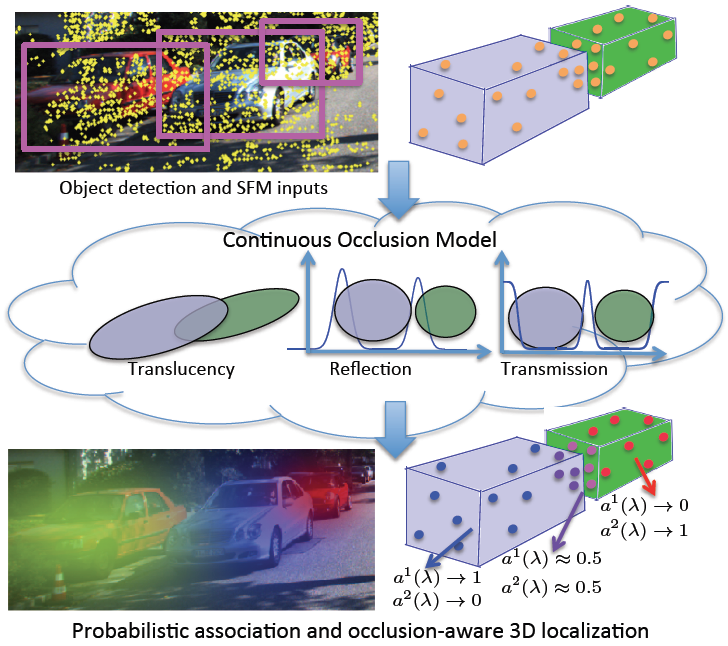
\includegraphics[width=\linewidth]{graphics/figure1.png}
\end{center}
\vspace{-0.6cm}
\caption{\small We propose an occlusion model in 3D that is physically-inspired and continuous. Given object detection and SFM point tracks, our unified model probabilistically assigns point tracks to objects and reasons about object detection scores and bounding boxes. It uniformly handles static and dynamic objects, thus, outperforms motion segmentation for association problems. We also demonstrate occlusion-aware 3D localization in road scenes.}
\label{fig:page1}
\vspace{-0.4cm}
\end{figure}

Our main contribution is a novel theoretical model for occlusion handling that is continuous and fully 3D. Our model is motivated by insights from computer graphics, whereby we represent objects as translucent 3D ellipsoids. In Section \ref{sec:setup}, we develop novel continuous models for representing \emph{transmission} and \emph{reflection} probabilities for each ray emanating from the camera. This allows assigning probabilities for each point in space belonging to an object, which can explicitly explain image observations and reason about occlusions. This is in contrast to prior works that consider occlusions in 2D, or through discrete occluder patterns or models that are not physically interpretable \cite{Pepik_etal_2012,Pepik_etal_2013,Xiang_Savarese_2013,Zia_etal_2013,Zia_etal_2014,Zia2015}.


A key advantage afforded by our occlusion model is unification. While previous approaches to handling occlusions are application-dependent, ours is physically-inspired, thus, flexible enough to be used in a variety of scenarios. In this paper, we show that our theory can be used for uniformly modeling the association of SFM point tracks with static or dynamic objects (Section \ref{sec:association}), as well as modeling object detection scores in applications like 3D localization (Section \ref{sec:localization}). We demonstrate the application of our formulations for road scenes from the KITTI raw dataset \cite{Geiger_etal_2012}.


In particular, assigning 2D point tracks to independent, but potentially occluding, objects is a fundamental challenge in computer vision problems such as multibody SFM \cite{Ozden_etal_2010}. Recent works use motion segmentation \cite{Brox_Malik_2010,Rao_etal_2010} as a precursor to localizing objects, which often suffices for moving objects \cite{Tron_Vidal_2007} and has also been considered for multibody SFM \cite{Kundu_etal_2011}. However, motion-based segmentation is not always applicable in road scenes, due to static parked cars, or dynamic cars that move with similar velocities. Occlusions make the problem more severe since point tracks get clustered together for static objects and may frequently appear to change association among dynamic objects in 2D.
%In contrast, we leverage the success of 
Indeed, we show in Section \ref{sec:experiments} that our point track association outperforms state-of-the-art motion segmentation methods, as well as a baseline that uses detection bounding boxes but does not consider occlusions.

Another potential application of our proposed model is towards 3D localization in road scenes. Prior works such as \cite{Song_Chandraker_2015} combine information from point tracks and detection bounding boxes, but do not consider occlusions for either. In contrast, our unified occlusion model allows a probabilistic soft assignment of point tracks to objects, as well as an occlusion-aware interpretation of object detection outputs. Our model is continuous, so it remains amenable to the use of continuous optimization tools.

To summarize, our main contributions are:
\vspace{-0.2cm}
\begin{tight_itemize}
%\setlength\itemsep{0cm}
\item A novel theoretical model for handling occlusions that is continuous and formulated in 3D.
\item Unified occlusion handling for point tracks in SFM and bounding boxes and detection scores in object detection.
\item Application of our model to association of point tracks with both static and moving objects, improving over motion segmentation and occlusion-unaware baselines.
\item Application of our unified formulation to 3D localization of traffic participants in road scenes.
\end{tight_itemize}



%A fundamental problem in computer vision is to separate feature points of multiple objects which are tracked through a video sequence. The assignments of point tracks to objects can serve as an important preprocessing step for different applications such as 3D localization and reconstruction, where the point tracks associated with an individual object can be used to localize or reconstruct the object in 3D space accurately. In this paper, we focus on road scenes in autonomous driving applications which often include dynamic and static objects simultaneously. For example, some cars are parked near the curb while other cars are moving on the street. 

%Motion segmentation approaches~\cite{Rao_etal_2010,Brox_Malik_2010} usually rely on object motions for clustering point tracks. Since point tracks of the same object possess similar motion patterns, these methods generally produce accurate point-to-object associations for dynamic objects~\cite{Tron_Vidal_2007}. However, when there are static objects in the scene, their corresponding point tracks are often clustered together, which decreases the performances significantly and makes motion segmentation approaches unsuitable for road scenes with combinations of dynamic and static objects. Moreover, object occlusions are frequently involved in road scenes, where cars are relatively close to each other and move in the same directions, which makes the problem of point-to-object association for road scene understanding become more challenging.

%In this work, we first propose to model objects as 3D ellipsoids. Motivated by image formulation theory in computer graphics, we then develop novel continuous models for representing \emph{transmission} and \emph{reflection} probabilities, which can explicitly explain image observations and reason about object occlusions. Leveraging on the success of object detection and tracking algorithms~\cite{Felzenszwalb_etal_2010,Choi_Savarese_2010}, we assume that detection bounding boxes and object tracklets are provided, thus we concentrate on segmenting point tracks that are computed only within object tracklets~\cite{Zach2007}, including both dynamic and static point tracks. As we will show in the experiments, the proposed continuous occlusion modelling method outperforms the baseline method which merely uses bounding boxes for dealing with occlusions. Furthermore, our method is not based on object motions and hence does not suffer from static objects as other state-of-the-art motion segmentation methods~\cite{Rao_etal_2010,Brox_Malik_2010}.

%As another important contribution, we examine the applicability of the proposed model for 3D localization in autonomous driving. In contrast to the bounding box baseline method, which uses hard assignments of point tracks to objects (i.e., $\{0,1\}$ probabilities), our continuous occlusion modelling method employs soft assignments (i.e., [$0,1$] probabilities). Consequently, it offers a \emph{unified} continuous occlusion modelling for both point track and bounding box energies, which allows the use of effective continuous optimization tools. As we will show later, the proposed model benefits the task of 3D localization in autonomous driving in terms of lower translation and dimension errors compared to those of~\cite{Song_Chandraker_2014}, which employs bounding boxes for point-to-object associations.

%The rest of the paper is organized as follows: Section~\ref{sec:related} discusses related work. Section~\ref{sec:setup} describes the proposed continuous occlusion model for road scene understanding. Section~\ref{sec:experiments} presents detailed experiments for point-to-object association and 3D localization. Finally, we conclude in Section~\ref{sec:conclusions}.

%The problem of segmenting points to objects often comes up in different computer vision problems especially in multi-body reconstruction and localization. Given correspondence points on consecutive frames, the problem becomes one of finding out which points belong to which object, following which one can use the consensus of segmented points to reconstruct or localize the object more accurately. Without additional information, this is a very difficult problem as attempted by semantic segmentation and motion segmentation methods. However, in the problems like reconstruction and localization one can use the hypothesis of the algorithm as the feedback.
% What is the problem we are trying to solve, and why is it even important?

% What did we do We propose a novel model for representation of objects in the scene so that point tracks can be probabilistically associated with objects while accounting for object occlusions.
% Why is it novel

%Although our proposed model is inspired by Milan et al.\cite{Milan_etal_2014}, it is more detailed and more principled than their work. Milan et al. used soft ellipses and sigmoids to model pedestrians and their occlusions. Our reasoning is instead in 3D. We use ellipsoids to model objects and reason about their occupancies of the space to model their occlusions.
% Ok you proposed a model is it of any use
% How does it compare to state of art
% We show that our continuous occlusion model achieves significantly lower point-to-object association errors compared to the baseline method using detection bounding boxes and other state-of-the-art methods for motion segmentation~\cite{Brox_Malik_2010, Rao_etal_2010}. As a consequence, our model benefits the task of 3D localization of traffic participants in autonomous driving.
